% Created 2019-04-26 Fri 10:06
% Intended LaTeX compiler: pdflatex
\documentclass[10pt,t,a4paper]{beamer}
\usepackage[utf8]{inputenc}
\usepackage[T1]{fontenc}
\usepackage{graphicx}
\usepackage{grffile}
\usepackage{longtable}
\usepackage{wrapfig}
\usepackage{rotating}
\usepackage[normalem]{ulem}
\usepackage{amsmath}
\usepackage{textcomp}
\usepackage{amssymb}
\usepackage{capt-of}
\usepackage{hyperref}
\usetheme{BTH_msv}
\author{Mikael Svahnberg\thanks{Mikael.Svahnberg@bth.se}}
\date{\today}
\title{Modelling Structure}
\hypersetup{
 pdfauthor={Mikael Svahnberg},
 pdftitle={Modelling Structure},
 pdfkeywords={},
 pdfsubject={},
 pdfcreator={Emacs 25.3.1 (Org mode 9.1.2)}, 
 pdflang={English}}
\begin{document}

\maketitle

\section{Classroom}
\label{sec:org4671b3d}
\begin{frame}[label={sec:orgc4aa964}]{Discussion: Concepts and Attributes}
\begin{itemize}
\item How can we find / What are:
\begin{itemize}
\item Concepts
\item Attributes
\item Associations
\end{itemize}
\item What is the difference between an \emph{Attribute} and a \emph{Concept}
\end{itemize}
\end{frame}
\begin{frame}[label={sec:org82f981b}]{Identifying Concepts}
\begin{center}
\begin{tabular}{lll}
Category & Examples & \\
\hline
Physical Objects & POST & Aeroplane\\
Places & Store & Aerport\\
Transactions & Payment & Reservation\\
Containers & Basket & Aeroplane\\
Things in Container & Item & Passenger\\
Events & Sale & Flight\\
Description of Things & Sale Item & Flight Description\\
Records, Contracts & Receipt & Ticket\\
\hline
\end{tabular}
\end{center}
\end{frame}
\begin{frame}[label={sec:orgabba7ae}]{Finding Concepts}
\begin{itemize}
\item Look for \emph{nouns}
\item Map nouns to concepts
\end{itemize}

Sources:     
\begin{itemize}
\item Textual description of problem domain
\item Requirements
\item Use-cases
\end{itemize}

Cave!
\begin{itemize}
\item Natural language is ambiguous
\item Concepts or Attributes?
\end{itemize}
\end{frame}

\begin{frame}[label={sec:org19541cd}]{Attributes}
\begin{itemize}
\item Logical value of an element
\begin{itemize}
\item Examples: \emph{name, quantity, status, \ldots{}}
\item Hint: Builtin data types
\begin{itemize}
\item String, int, date
\item But also simple user-defined types such as \emph{address, personnummer, \ldots{}}
\end{itemize}
\end{itemize}
\item \alert{Keep Attributes Simple}
\end{itemize}
\end{frame}
\begin{frame}[label={sec:org18387f3}]{Associations}
An association is a
\begin{itemize}
\item relationship between concepts
\item indicates a meaningful and interesting connection
\end{itemize}

Types
\begin{itemize}
\item Need-to-know (preserved for some time; needs to maintained by software)
\item Comprehension-only (used to understand domain)
\end{itemize}
\end{frame}
\begin{frame}[label={sec:org9108201}]{Finding Associations}
\begin{center}
\begin{tabular}{ll}
Category & Examples\\
\hline
A -- is a part of -- B & Salesitem -- Sale\\
 & Wing -- Aeroplane\\
A -- is contained in -- B & Item -- Store\\
 & Seat -- Flight\\
A -- is a description for -- B & ItemDescription -- Item\\
 & FlightInformation -- Flight\\
A -- is known/recorded in -- B & Sale -- POST\\
 & Booking -- Flight\\
A -- is owned by -- B & Store -- Company\\
A -- related transactions -- B & Payment -- Sale\\
 & Booking -- Ticket\\
\hline
\end{tabular}
\end{center}
\end{frame}
\begin{frame}[label={sec:org37e2b4c}]{Discussion: Multiplicity}
\begin{itemize}
\item Go through different types of multiplicity
\end{itemize}
\end{frame}
\begin{frame}[label={sec:org3aa1e25}]{Discussion: Concept or Class}
\begin{itemize}
\item When does a conceptual diagram become a class diagram?
\end{itemize}
\end{frame}
\begin{frame}[label={sec:org33916c7}]{Aggregation}
\begin{itemize}
\item Aggregation
\begin{itemize}
\item ``Has-a''
\item Strong aggregation
\end{itemize}
\item Composition
\begin{itemize}
\item ``Consists-of''
\item weak aggregation
\end{itemize}
\end{itemize}

\begin{center}
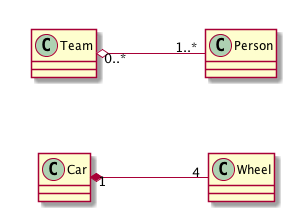
\includegraphics[height=4cm]{FAggregation2.png}
\end{center}
\end{frame}
\begin{frame}[label={sec:orgf5bfe4d}]{Discussion: An Example}
\begin{center}
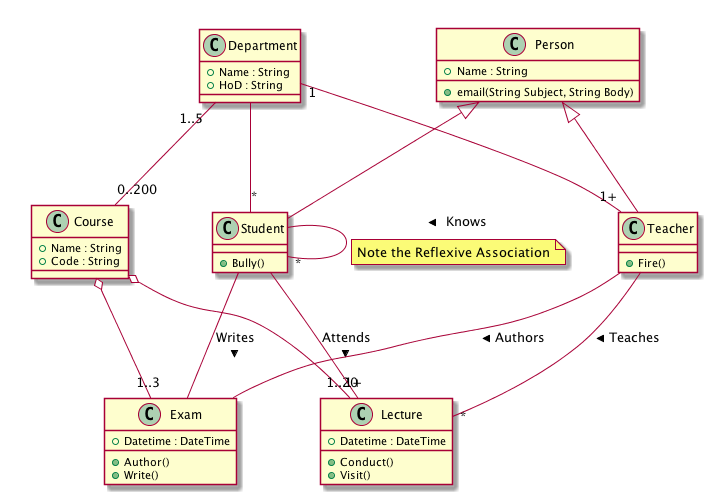
\includegraphics[height=6.5cm]{FExampleUniversity.png}
\end{center}
\end{frame}
\begin{frame}[label={sec:org0e2c1e7}]{Example}
\begin{itemize}
\item Conceptual Model for Discussion Forum Software
\end{itemize}
\end{frame}
\begin{frame}[label={sec:orge11461d}]{Generalisation (Inheritance)}
Why
\begin{itemize}
\item Classification among concepts (is-a)
\item Code reuse, identifying commonalities
\end{itemize}

Example
\begin{itemize}
\item Vector Graphics Drawing Programme
\begin{itemize}
\item Point, Line, Arc, Polygon, Ellipse, Circle
\end{itemize}
\end{itemize}
\end{frame}
\begin{frame}[label={sec:org91e3b5f}]{Generalisation: Hierarchy}
\begin{center}
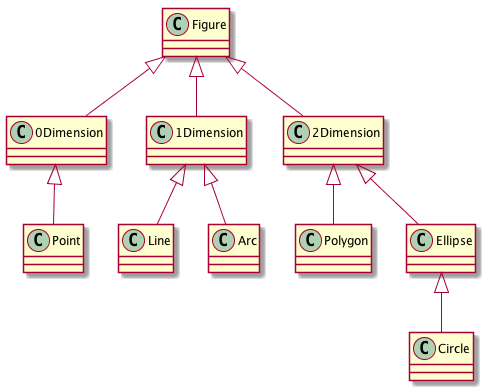
\includegraphics[height=6.5cm]{FInheritance.png}
\end{center}
\end{frame}

\begin{frame}[label={sec:orgb0f2925}]{Generalisation: Hierarchy II}
\begin{center}
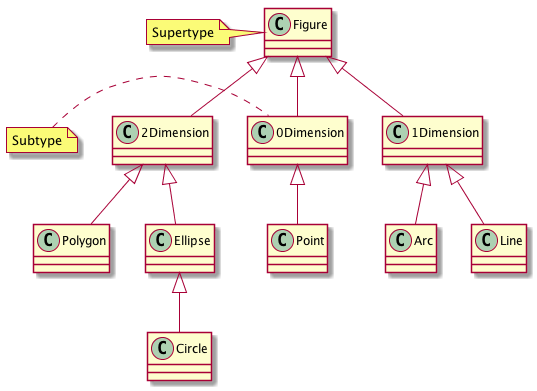
\includegraphics[height=6.5cm]{FInheritance2.png}
\end{center}
\end{frame}

\begin{frame}[label={sec:org0a9ead5}]{Generalisation: Hierarchy III}
\begin{center}
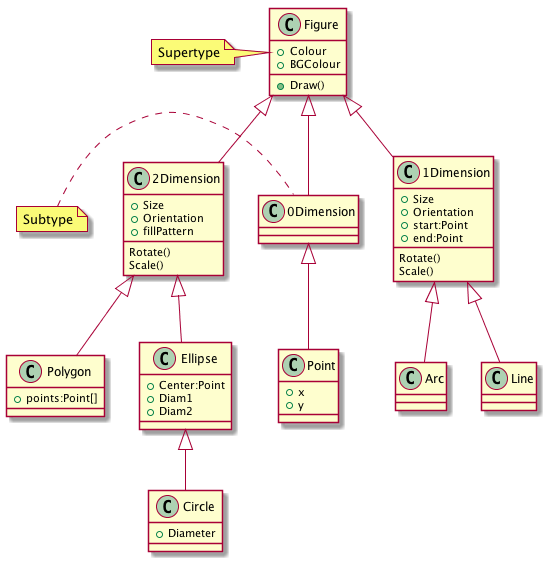
\includegraphics[height=6.5cm]{FInheritance3.png}
\end{center}
\end{frame}

\begin{frame}[label={sec:org857167a}]{Abstract Types}
\begin{itemize}
\item When no instances of the base class are desirable.
\item Example: There are no instances of the generic ``Figure'' base class.
\end{itemize}
\begin{center}
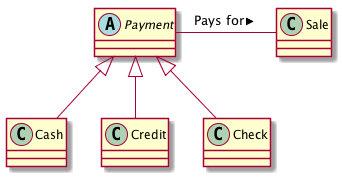
\includegraphics[height=4cm]{FInheritanceAbstract.png}
\end{center}
\end{frame}

\begin{frame}[label={sec:org394fff4}]{Reflexive Associations}
\begin{center}
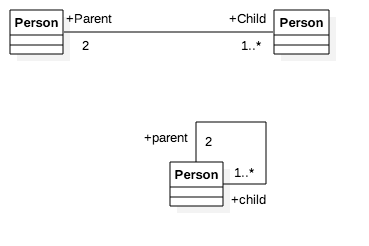
\includegraphics[width=.9\linewidth]{./IReflexive.png}
\end{center}
\end{frame}
\begin{frame}[label={sec:org2bd13fa}]{Exotic UML: Association Attributes}
\only<1>{
\begin{center}
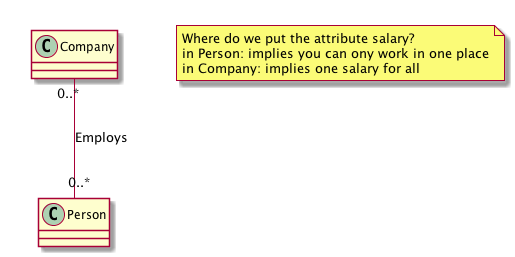
\includegraphics[height=6cm]{FAssociationAttributes0.png}
\end{center}
}


\only<2>{
One solution:

\begin{center}
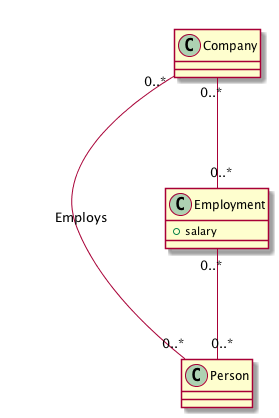
\includegraphics[height=6cm]{FAssociationAttributes1.png}
\end{center}
}


\only<3>{
Proper Solution:

\begin{center}
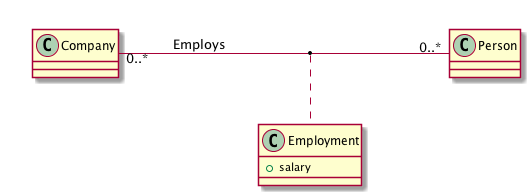
\includegraphics[width=10cm]{FAssociationAttributes2.png}
\end{center}
}
\end{frame}
\end{document}